\section{TANGENT ACTION MODEL FOR GROUP AVOIDANCE}
\label{sec:methods}

\subsection{Problem Formulation and Group Detection}

Our objective is to enable a robot to navigate to its goal while respecting both individual humans and group formations in dynamic environments. We formulate this as a conditional decision problem where the robot adapts its behavior based on real-time detection of human groups.

\UT{Try to address the 4th review of reviwer 31289}Rather than assuming perfect group knowledge, we employ spatial clustering for real-time group detection. At each timestep, we identify groups using DBSCAN with adaptive parameters: proximity threshold $\epsilon = 1.5$m and minimum group size of 2. Groups are detected based on spatial proximity and velocity alignment:

\begin{equation}
G_j = \{h_i | d(h_i, h_k) < \epsilon, |\mathbf{v}_i - \mathbf{v}_k| < v_{thresh}, \forall h_k \in G_j\}
\end{equation}

where $d(h_i, h_k)$ is the Euclidean distance between humans and $v_{thresh}$ is the velocity difference threshold for cohesive movement.

The robot observes the environment state $s_t$ comprising robot features $w_t$ (position, velocity, goal), individual humans $\{u_i^t\}_{i=1}^n$, and detected groups $\{g_j^t\}_{j=1}^m$:

\begin{equation}
s_t = \{w_t, u_1^t, ..., u_n^t\} \cup \{g_1^t, ..., g_m^t\}
\end{equation}

Each detected group $g_j^t$ is characterized by its centroid $C$, radius $R$, and member count $m_g$, where $C = \frac{1}{|G_j|}\sum_{h_i \in G_j} p_i$ and $R = \max_{h_i \in G_j} ||p_i - C||$.

\begin{figure}[!t]
\centering
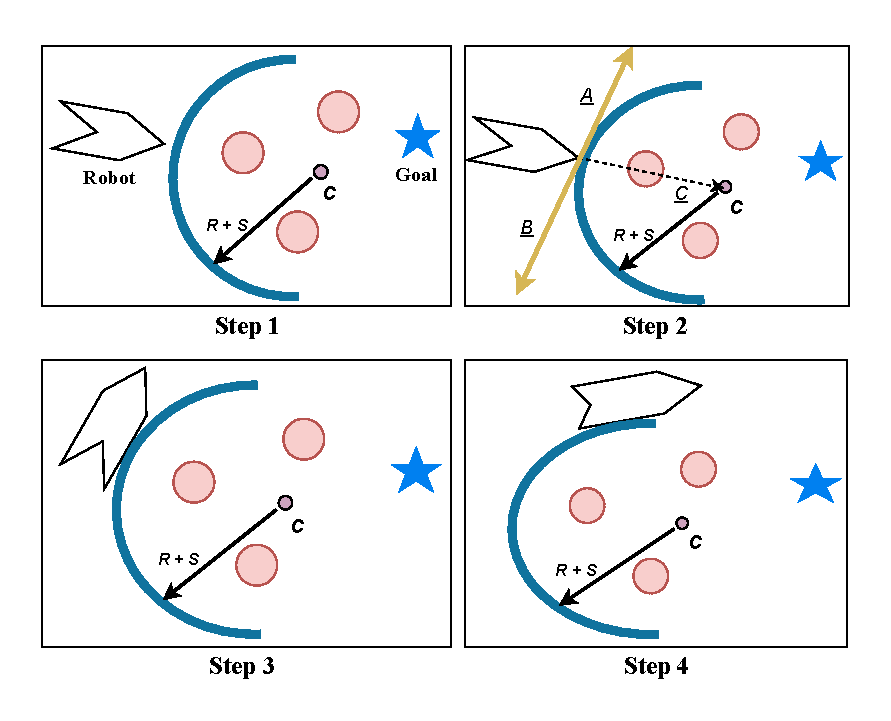
\includegraphics[width=3.5in]{figures/taga.pdf}
\caption{Visualization of the proposed TAGA process. The robot detects a human group with centroid $C$ and radius $R$. When the robot reaches switching distance $R+S$ from the centroid (where $S$ is the safety margin), TAGA activates and computes tangent trajectories. The robot navigates along the circular boundary at distance $R+S$ from $C$, selecting between clockwise and counterclockwise paths based on goal direction and safety constraints. Once past the group, TAGA deactivates and returns control to the baseline navigation policy.\UT{Step description require}}
\label{fig:taga-process}
\end{figure}

\subsection{Tangent-Based Navigation with Safety Guarantees}
\UT{Try to address the 3rd review of reviwer 31281 of safety concerns of individuals}
TAGA activates when the robot approaches a detected group within switching distance $R + S$ from the group centroid, where $R$ is the group radius and $S$ is a safety margin (typically 0.5m) beyond the group boundary. As illustrated in Figure \ref{fig:taga-process}, when $d(r, C) \leq R + S$, the robot computes a tangent trajectory that maintains this safe distance from the centroid. The tangent point on the circular boundary is:

\begin{equation}
p_T = C + (R + S) \cdot \hat{t}
\end{equation}

where $\hat{t}$ is the unit tangent vector. The robot selects between clockwise and counterclockwise tangent directions:

\begin{equation}
\hat{t} = \arg\min_{t \in \{t_{cw}, t_{ccw}\}} \left( w_1 \cdot \angle(t, \vec{g}) + w_2 \cdot d_{obs}(t) \right)
\end{equation}

where $\angle(t, \vec{g})$ measures angular deviation from the goal direction and $d_{obs}(t)$ accounts for obstacles along the tangent path.

To ensure individual collision avoidance during group maneuvers, we implement a hierarchical safety controller with graduated response zones:

\begin{equation}
a_{final} = \begin{cases}
    a_{stop} & d_{min} < d_{critical} \\
    \alpha a_{TAGA} + (1-\alpha) a_{avoid} & d_{critical} \leq d_{min} < d_{personal} \\
    a_{TAGA} & d_{min} \geq d_{personal}
\end{cases}
\end{equation}

where $d_{min} = \min_i d(r, h_i)$., $d_{critical} = 0.3$m triggers emergency stop, $d_{personal} = 0.5$m initiates blended avoidance, and:
\begin{equation}
\alpha = \frac{\min_i d(r, h_i) - d_{critical}}{d_{personal} - d_{critical}}
\end{equation}
provides smooth transitions between behaviors. This ensures that while navigating around groups at distance $R+S$, the robot maintains safe distances from any individuals who may be near but outside the detected group.

\subsection{Integration and Switching Mechanism}

\UT{Try to address the 2nd review of reviwer 31289}TAGA operates as a modular enhancement to existing navigation methods. Given a baseline navigation model $M$ (either reactive or learned), the integrated system follows:

\begin{equation}
\pi(s_t) = \begin{cases}
    \text{TAGA}(s_t) & \text{if group detected AND} \\
    & d(r, C) \leq R + S \text{ AND approaching} \\
    M(s_t) & \text{otherwise}
\end{cases}
\end{equation}

% The complete activation condition ensures TAGA engages only when necessary:

% \begin{equation}
% \text{activate} = (d(r, C) \leq R + S) \land (\vec{v}_r \cdot \vec{rC} > 0) 
% % \land (\text{conf} > \tau)
% \end{equation}

% where $\vec{v}_r$ is robot velocity, $\vec{rC}$ is the vector from robot to group centroid, and $\tau$ is the detection confidence threshold. The approaching condition $(\vec{v}_r \cdot \vec{rC} > 0)$ prevents unnecessary activation when moving away from groups.

% Deactivation occurs when the robot moves beyond $(R + S) + \delta$ from the centroid, where hysteresis margin $\delta = 0.2$m prevents oscillation between modes. The modular design preserves the baseline model's performance for individual interactions while adding group awareness without retraining. 

% Computational overhead remains minimal with $O(n \log n)$ for group detection and $O(k)$ for tangent computation across $k$ groups, enabling real-time operation at 10Hz. This integration approach allows TAGA to enhance any existing navigation framework—demonstrated through successful integration with ORCA, Social Force, DS-RNN, and AG-RL—while maintaining their original capabilities for scenarios without groups.

% \section{Tangent Action Model for Group Avoidance}

%  \begin{figure}[t]
%     \centering
%     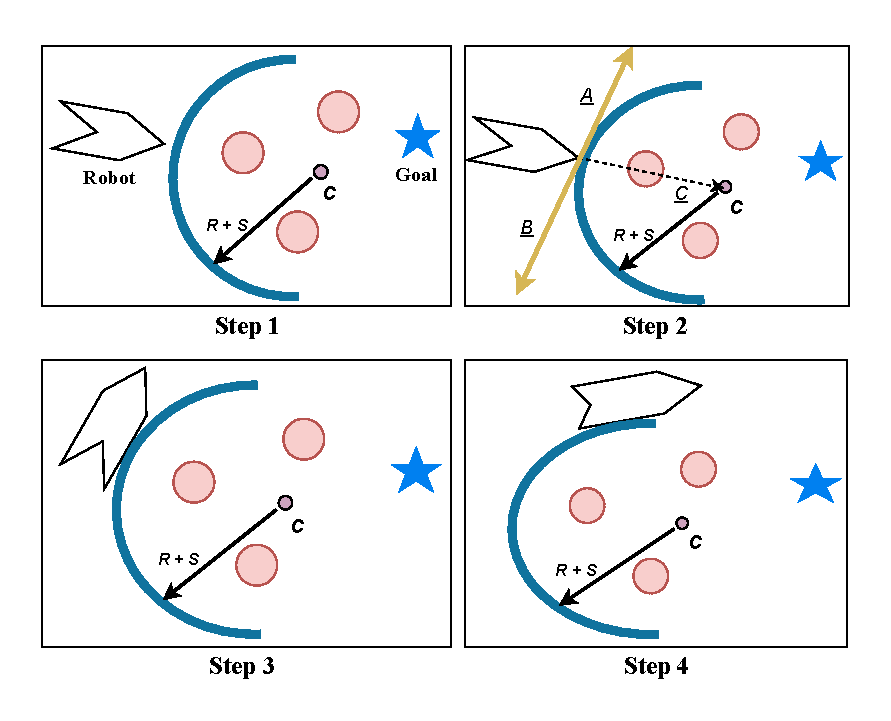
\includegraphics[scale=0.5]{figures/taga.pdf}
%     \caption{The Visualization of our proposed TAGA process. The robot, initially following a standard navigation model, detects a human group and activates TAGA. The model computes a tangent action based on the group centroid and boundary, enabling the robot to smoothly navigate around the group while ensuring social compliance. Once the group is passed, TAGA deactivates, allowing the robot to resume its default navigation policy towards the goal.}
%     \vspace{-15pt} 
%     \label{fig:taga}
% \end{figure}

% \subsection{Problem Formulation}
% Our objective is to learn a controller that allows a robot to navigate to a desired goal while maintaining social norms and avoiding collisions with individual pedestrians, human groups, and their boundaries. We formulate our approach using a reactive methodology. If the robot detects a group $G = \{ u_1, u_2, ..., u_m \}$, where $m$ is the number of group members, it activates its reactive nature.

% From a certain distance $S$, the robot adjusts its action to follow a tangent trajectory from the group's centroid to the robot's intercept point. This tangent action ensures smooth and socially compliant navigation while respecting group formations. Once the robot crosses the point where its distance to the group is less than the sum of the group’s radius, $r_g$ and a safety margin, $d_{\text{safe}}$, it deactivates its tangent behavior and resumes its default navigation strategy.
% % Once the robot crosses the group boundary, it deactivates its tangent behavior and resumes its default navigation strategy.

% \vspace{-5pt} 
% \subsection{State and Action Representation}
% % We model the navigation task as a decision-making process where the robot must reach a goal while avoiding collisions with individual humans and human groups. At each timestep $t$, the robot observes the environment and selects an action accordingly.

% % Following \cite{liu2023intention}, the state $s_t$ is represented as:

% % % $$
% % % s_t = \left[ w^t, \mathbf{u}_1^t, \hat{\mathbf{u}}_1^{t+1:t+K}, ..., \mathbf{u}_n^t, \hat{\mathbf{u}}_n^{t+1:t+K} \right] \eqno{(6)}
% % % $$
% % \begin{equation}
% % s_t = \left[ w^t, \mathbf{u}_1^t, \hat{\mathbf{u}}_1^{t+1:t+K}, ..., \mathbf{u}_n^t, \hat{\mathbf{u}}_n^{t+1:t+K} \right]
% % \end{equation}


% % where $w^t$ includes global features such as the robot’s position, velocity, and goal. Each human $i$ is represented by $\mathbf{u}_i^t = (p_i, v_i)$, which denotes their position and velocity, while $\hat{\mathbf{u}}_i^{t+1:t+K}$ captures predicted future states over the next $K$ timesteps. The number of humans $n$ varies dynamically over time.

% % To incorporate human group dynamics, we extend this representation by introducing additional group-level observations:

% % % $$
% % % s_t = s_t \cup \{ g_1^t, g_2^t, ..., g_m^t \} \eqno{(7)}
% % % $$
% % \begin{equation}
% % s_t = s_t \cup \{ g_1^t, g_2^t, ..., g_m^t \}
% % \end{equation}

% % where each group $j$ is described as:

% % % $$
% % % g_j^t = (c_g^j, r_g^j, m_g^j, \text{group\_id}^j)
% % % $$
% % \begin{equation}
% % g_j^t = (c_g^j, r_g^j, m_g^j, \text{grp\_id}^j, \{ \text{h\_id}_1, \text{h\_id}_2, ..., \text{h\_id}_{m_g^j} \})
% % \end{equation}

% % % Here, $c_g^j$ and $r_g^j$ denote the centroid and radius of the group, $m_g^j$ represents the number of members, and $\text{group\_id}^j$ is a unique identifier. The total number of groups $m$ varies based on crowd formations.
% % Here, $c_g^j$ and $r_g^j$ denote the centroid and radius of the group, which define the group's spatial representation, $m_g^j$ represents the number of members in the group, $\text{grp\_id}^j$ is a unique identifier assigned to each group, $\{ \text{h\_id}_1, \text{h\_id}_2, ..., \text{h\_id}_{m_g^j} \}$ represents the set of human IDs belonging to the group, ensuring the robot can track individual members within a group. The total number of groups $m$ varies dynamically based on crowd formations, allowing the system to adapt to real-world human interactions.


% % The action at each timestep is given by $a_t = (v_x, v_y)$, where $v_x$ and $v_y$ define the robot’s velocity along the x and y axes, respectively. The robot follows holonomic kinematics, allowing unrestricted movement in any direction.
% We model navigation as a decision-making process where the robot must reach its goal while avoiding collisions with individuals and human groups. At each timestep \( t \), the robot observes the environment and selects an action.

% Following \cite{liu2023intention}, the state \( s_t \) is represented as:
% % \vspace{-10pt} % Reduce space before
% \begin{equation}
% s_t = \left[ w^t, \mathbf{u}_1^t, \hat{\mathbf{u}}_1^{t+1:t+K}, ..., \mathbf{u}_n^t, \hat{\mathbf{u}}_n^{t+1:t+K} \right] \cup \{ g_1^t, g_2^t, ..., g_m^t \}
% \end{equation}
% % \vspace{-12pt} % Reduce space before
% where \( w^t \) includes global robot features (position, velocity, goal), and each human \( i \) is represented by \( \mathbf{u}_i^t = (p_i, v_i) \), with \( \hat{\mathbf{u}}_i^{t+1:t+K} \) predicting future states over \( K \) timesteps. The number of humans \( n \) varies dynamically.

% Each group \( j \) is defined as:

% \vspace{-8pt} % Reduce space before
% \begin{equation}
% g_j^t = (c_g^j, r_g^j, m_g^j, \text{grp\_id}^j, \{ \text{h\_id}_1, ..., \text{h\_id}_{m_g^j} \})
% \end{equation}
% % \vspace{-8pt} % Reduce space before
% where \( c_g^j \) and \( r_g^j \) are the group centroid and radius, \( m_g^j \) is the number of members, and \( \text{grp\_id}^j \) is a unique identifier. The set \( \{ \text{h\_id}_1, ..., \text{h\_id}_{m_g^j} \} \) tracks individual members, allowing dynamic adaptation to crowd formations.

% The action at each timestep is $a_t = (v_x, v_y)$, where $v_x$ and $v_y$ define the robot’s velocity in a holonomic kinematic model.


% \subsection{Tangent Action Model}
% To enable group-aware navigation, we propose a tangent-based action model, TAGA, that allows the robot to smoothly bypass human groups while progressing toward its goal. Unlike traditional avoidance mechanisms that only consider individual humans, our approach ensures that the robot respects the spatial integrity of human groups by following a tangent trajectory around them.

% \subsubsection{Tangent Computation}
% % Given a detected group $G = \{ u_1, u_2, ..., u_m \}$, where $m$ is the number of group members, the group is represented by a centroid $c_g$ and a radius $r_g$:

% % \begin{equation}
% % c_g = \frac{1}{m} \sum_{i=1}^{m} p_i, \quad r_g = \max_{i} \| p_i - c_g \|
% % \end{equation}


% % where $p_i = (x_i, y_i)$ represents the position of the $i$-th group member. 

% % The robot, positioned at $p_r = (x_r, y_r)$, adjusts its trajectory when it reaches a switching distance $S$ from the group's boundary:

% % \begin{equation}
% % S = r_g + d_{\text{safe}}
% % \end{equation}

% % where $d_{\text{safe}}$ is a safety margin to prevent near-collisions.

% Given a detected group $G = \{ u_1, u_2, ..., u_m \}$, where $m$ is the number of members, the group is represented by a centroid $c_g  = \frac{1}{m} \sum_{i=1}^{m} p_i$ and a radius, $r_g = \max_{i} \| p_i - c_g \|$, and the switching distance $S = r_g + d_{\text{safe}}$,  
% where $p_i = (x_i, y_i)$ is the position of the $i$-th member, and $d_{\text{safe}}$ is a safety margin to prevent near-collisions. The robot, positioned at $p_r = (x_r, y_r)$, adjusts its trajectory when it reaches $S$ from the group boundary.

% At this point, the robot selects one of the tangent points $(p_T)$ on the group’s boundary as its temporary subgoal:

% % $$
% % p_T = c_g + r_g \cdot \hat{t} \eqno{(11)}
% % $$
% \vspace{-10pt}
% \begin{equation}
% p_T = c_g + r_g \cdot \hat{t}
% \end{equation}

% where $\hat{t}$ is the unit tangent direction from the robot to the group boundary. The tangent is computed based on the relative position of the robot and the group centroid.

% \subsubsection{Tangent Navigation Process}
% % As shown in Fig. \ref{fig:taga}, the robot follows these steps:

% % \begin{enumerate}
% %     \item \textbf{Detection:} The robot identifies a human group and calculates its centroid and boundary.
% %     \item \textbf{Switching Activation:} Once within the switching distance $S$, the robot activates the tangent avoidance mechanism.
% %     \item \textbf{Tangent Selection:} The robot computes the tangent trajectory and selects the optimal path around the group.
% %     \item \textbf{Reintegration:} After crossing the group boundary, the robot deactivates the tangent behavior and resumes direct goal navigation.
% % \end{enumerate}
% As shown in Fig. \ref{fig:taga}, the robot follows a structured process for group-aware navigation. First, it detects a human group and calculates its centroid and boundary. When it reaches the switching distance $S$, the tangent avoidance mechanism is activated. The robot then computes the tangent trajectory and selects the optimal path around the group. Once it crosses the group boundary, it deactivates the tangent behavior and resumes direct goal navigation.

% % By incorporating these reactive adjustments, the robot avoids unnatural or abrupt maneuvers, ensuring a smooth and socially compliant navigation strategy. The proposed model can be easily integrated into existing navigation frameworks to enhance group-awareness while leveraging pre-trained policies designed for individual-based navigation.

% \subsection{Implementation Details}
% Our proposed TAGA model is designed to integrate seamlessly with existing navigation models, particularly those trained on environments with individual humans. A navigation model $M$ represents either a learning-based policy trained on individual pedestrian interactions or a reactive method optimized for avoiding individual humans.

% To ensure socially compliant navigation in the presence of human groups, TAGA operates as a conditional module that activates only when a group is detected. The navigation policy follows a switching mechanism, where the robot's action selection is based on the observed state $s$:

% % $$
% % f(s) =
% % \begin{cases} 
% %     \text{TAGA}(s), & \text{if a human group is detected} \\
% %     M(s), & \text{otherwise}
% % \end{cases} \eqno{(12)}
% % $$
% \vspace{-8pt} % Reduce space before
% \begin{equation}
% f(s) =
% \begin{cases} 
%     \text{TAGA}(s), & \text{if a human group is detected} \\
%     M(s), & \text{otherwise}
% \end{cases}
% \end{equation}


% where, $s$ represents the robot's current state, including its position, velocity, and the surrounding human configuration, $M(s)$ outputs an action based on the baseline navigation model in environments without groups, $\text{TAGA}(s)$ computes a tangent action when a group is detected, adjusting the robot's trajectory for socially compliant navigation, $f(s)$ represents the final action executed by the robot.

% % \begin{figure*}[t]
% %     \centering
% %     \resizebox{\textwidth}{!}{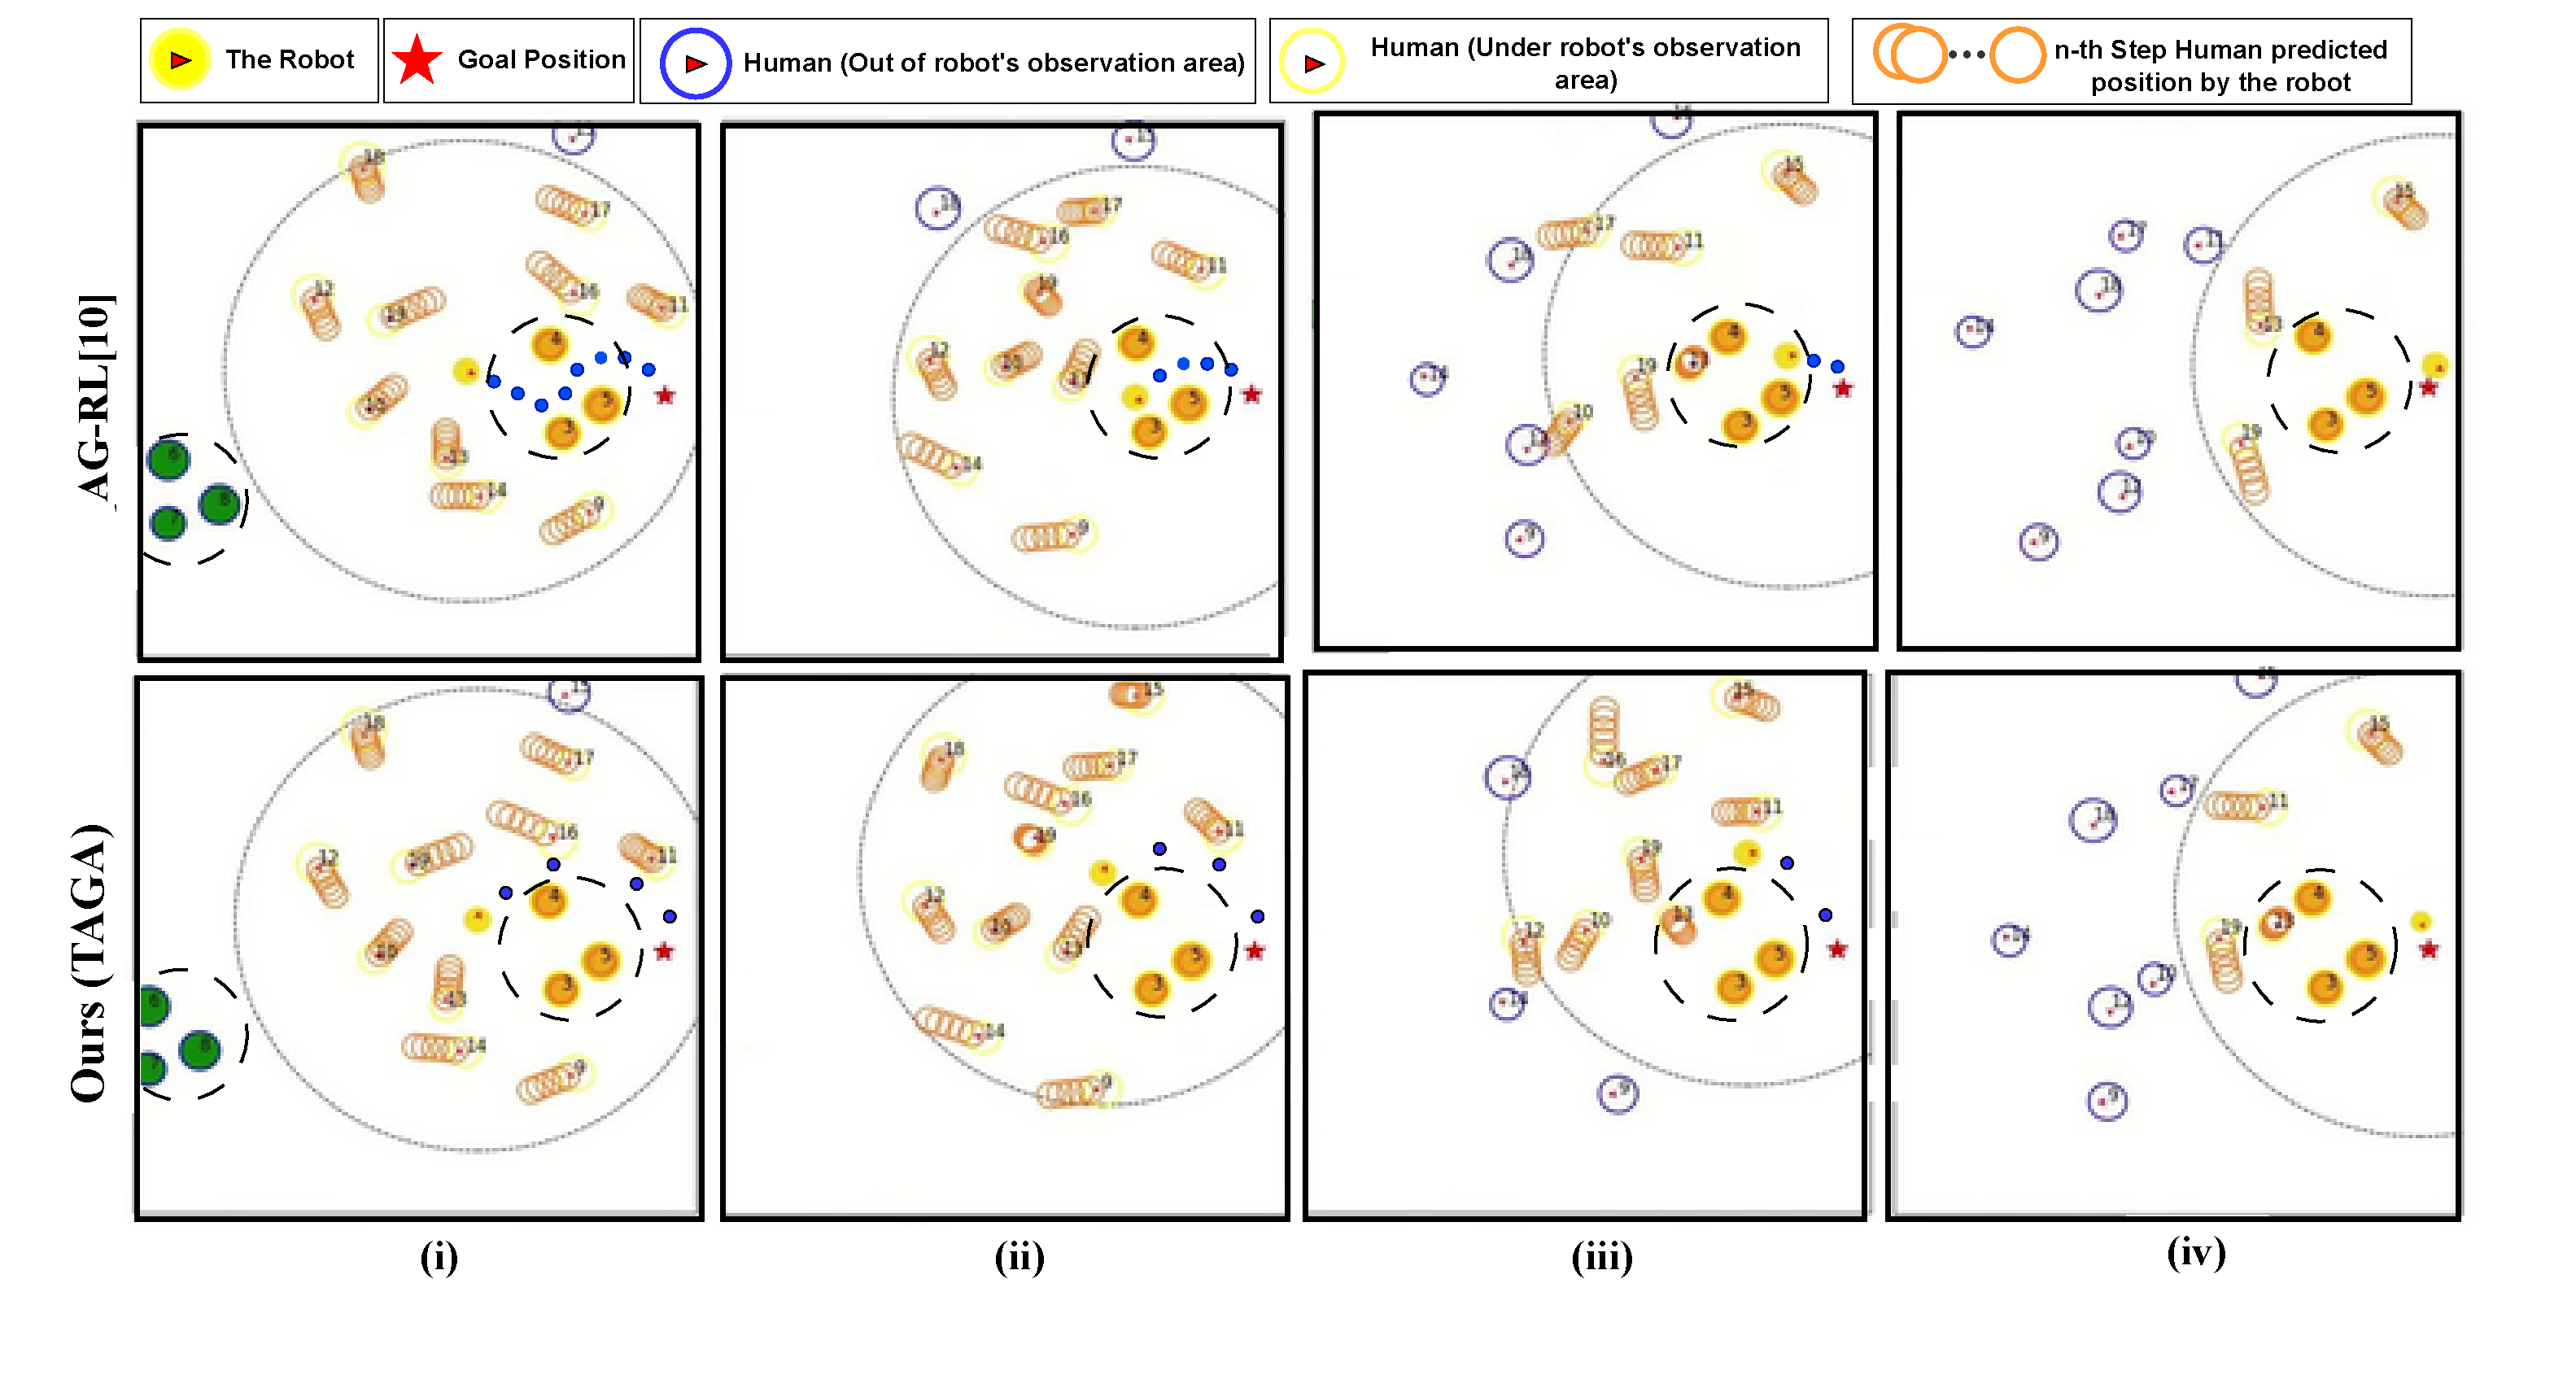
\includegraphics{figures/com.pdf}}
% %     \vspace{-25pt}
% %     \caption{\textbf{Comparison of our method (TAGA) and the state-of-the-art approach during the same testing episode, with identical randomized human and group placements.} The dotted circles represent group boundaries, while the small blue dots illustrate the robot's trajectory towards its goal. To ensure uninterrupted navigation, group collision constraints were disabled during the episode, allowing for continuous observation of the robot’s path planning and decision-making behavior.
% % }
% %     \vspace{-15pt}  
% %     \label{fig:sim-com}
% % \end{figure*}


% The integration of TAGA with an existing model $M$ follows a reactive approach based on group detection. \UT{The robot continuously monitors its surroundings and identifies human groups using spatial clustering, where group membership is determined by the proximity of individuals. Additionally, the robot calculates the average velocity of group members to identify cohesive movement patterns, further refining the group detection process.} If no group is detected, the robot follows the original navigation model $M(s)$, which provides actions for avoiding individual pedestrians. However, when a group is identified, the control switches to TAGA, which adjusts the robot’s trajectory using a tangent-based avoidance strategy. TAGA computes a path around the group boundary to ensure smooth and socially compliant navigation. Once the robot successfully passes the group, TAGA deactivates, and the control returns to $M(s)$, allowing the robot to resume its default navigation behavior.

% This modular design ensures that TAGA does not interfere with pre-trained policies when no groups are present, making it adaptable to any existing navigation model. The proposed approach effectively allows individual-based navigation frameworks to inherit group-awareness without retraining the entire model, thereby improving real-world applicability.
